\documentclass[letter]{article}

\usepackage{amsmath,amsfonts}

\setlength{\oddsidemargin}{0in}
\setlength{\textwidth}{6in}
\setlength{\topmargin}{0in}
\setlength{\headheight}{0in}
\setlength{\headsep}{0in}
\setlength{\textheight}{8.7in}
\usepackage[english]{babel}
\usepackage[utf8x]{inputenc}
\usepackage{amsmath}
\usepackage{graphicx}
\usepackage[colorinlistoftodos]{todonotes}
% \usepackage{biblatex}
\usepackage{booktabs}
\usepackage{array}
\usepackage{boxedminipage}
\usepackage{subfigure}
\large
\title{Assignment1: Decision Trees}
\author{Xiao Liu}

\begin{document}
\maketitle
\section{Dataset Description}
The dataset is from UCI machine learning directories. These are real word 
data collected by Paulo Cortez (Univ. Minho) and Sérgio Moro (ISCTE-IUL) 
\cite{moro2011using}. These real-world data were collected from a Portuguese
marketing campaign related with bank deposit subscription. The business goal
is to find a model that can explain success of a contact, i.e. if the client
subscribes the deposit. Such model can increase campaign efficiency by
identifying the main characteristics that affect success, helping in a 
better management of the available resources (e.g. human effort, phone 
calls, time) and selection of a high quality and affordable set of potential
buying customers. The marketing campaigns were based on phone calls. Often, 
more than one contact to the same client was required, in order to access if 
the product (bank term deposit) would be (or not) subscribed. 

There are 45211 instances in the original data set and we applied 10\%, that
is 4521 instances, for this task by random sampling. Basically, this is a 
binary classification task that we use in total 16 attributes to predict 
``{\bf Whether a person will subscribe the deposit}''. The 16 input 
variables/attributes and their details are listed in Table~\ref{table1}.

\begin{table*}[!htbp]
\centering
\caption{Attributes and Description}\label{table1}
\begin{tabular}{l}
\hline
\hline
Attributes: Descriptions\\
\midrule
age : numeric\\
type of job : categorical: ``admin.'',``unknown'',...,``unemployed''\\
marital status : categorical: ``married'',``divorced'',``single''\\
education :categorical : ``unknown'',``secondary'',``primary'',``tertiary''\\
has credit in default? : binary: ``yes'',``no''\\
average yearly balance, in euros : numeric\\
has housing loan? : binary: ``yes'',``no''\\
contact communication type : categorical: ``unknown'',``telephone'',``cellular''\\
last contact day of the month : numeric\\
last contact month of year : categorical: ``jan'', ``feb'', ..., ``nov'', ``dec''\\
last contact duration, in seconds : numeric\\
number of contacts performed during this campaign : numeric\\
number of days that passed by after the client was last contacted : numeric\\
number of contacts performed before this campaign : numeric\\
outcome of the previous campaign : categorical: ``unknown'',``other'',``failure'',``success''\\
\hline
\hline
\end{tabular}
\end{table*}


\section{Model Fit}
We conducted experiments to evaluate the performance of the decision trees 
under varying conditions for classifying the people into two categories: 
``yes'' for ``Subscription'' and ``No'' for ``Non-Subscription''. In order 
to build a prediction model and test it, we separate the data into the 
``Training Set'' and ``Testing Set'' by ratio of 7:3. We first fitted the 
data in the training set with an unbounded tree by setting up the elements
in the model as shown in Table~\ref{setting}. Then we used cross-validation
to prune this large tree with 47 splits based on the the relationship 
between the corresponding errors and the number of splits.

\subsection{Full Tree}
To grow a full tree, our algorithm made use of the Gini criterion for
choosing splits, with 2 observations necessary in each split. The default
setting for the parameters are indicated in Table~\ref{setting}. We use 70\%
of the data, that is 3181 instances, from the complete data set for training
this tree. As a result, we grow a tree with 47 splits to achieve the stopping
criteria, that is Complexity Parameter=0 as we configured.

\begin{table*}[!htbp]
\centering
\caption{Settings}\label{setting}
\begin{tabular}{ll}
\hline
\hline
Goodness of splits& Gini Index\\
Stopping criteria& All leaves are pure\\
&or all leaves contain less than 2 samples.\\
Class assignment& Yes or No\\
\hline
\hline
\end{tabular}
\end{table*}

\begin{figure}[!tp]
\centering
\includegraphics[width=1\columnwidth]{fig/fulltree}
\caption{Full Tree}
\label{full}
\end{figure}  


\begin{table*}[!htbp]
\centering
\caption{Splits Results}\label{split}
\begin{tabular}{lllll}
\hline
\hline
Complexity Parameter& nsplit & error & xerror & xstd \\
\hline
0.029255319   &   7& 0.8617021 &0.9654255 &0.04769294\\
0.018617021    &  9& 0.8324468 &0.8936170 &0.04610426\\
0.013962766 &     11& 0.8138298 &0.8989362 &0.04622502\\
0.013297872  &    13& 0.7579787 &0.9095745 &0.04646501\\
\textbf{0.010638298}  &   \textbf{17}& \textbf{0.7313830} &\textbf{0.8989362}
 &\textbf{0.04622502}\\
0.009308511  &   19& 0.7101064 &0.9308511 &0.04693905\\
0.007978723  &   22& 0.6914894 &0.9361702 &0.04705634\\
0.006648936  &   24& 0.6755319 &0.9202128 &0.04670301\\
0.005319149  &   29& 0.6622340 &0.9202128 &0.04670301\\
\hline
\hline
\end{tabular}
\end{table*}

\begin{figure}[!tp]
\centering
\includegraphics[width=1\columnwidth]{fig/fit1-split}
\caption{Relative Error vs \#Splits}
\label{es}
\end{figure}

\subsection{Pruned Tree}
As can be seen in Table~\ref{split}, pruning of the decision tree is 
necessary since the tree is overfit. To make it clear, we also plot the
relationship between the Relative Error and number of Split in Figure~\ref{es}.
Obviously, we can find that, the Relative Error gets the minimum value when
there are in total 17 splits and the corresponding CP value is 0.010638298.
Taking advantage of this information, we pruned the full tree and demonstrate
the pruned tree in Figure~\ref{ptree}. In the pruned tree, there are in
total 17 splits which is much less than the fully developed tree.

\begin{figure}[!tp]
\centering
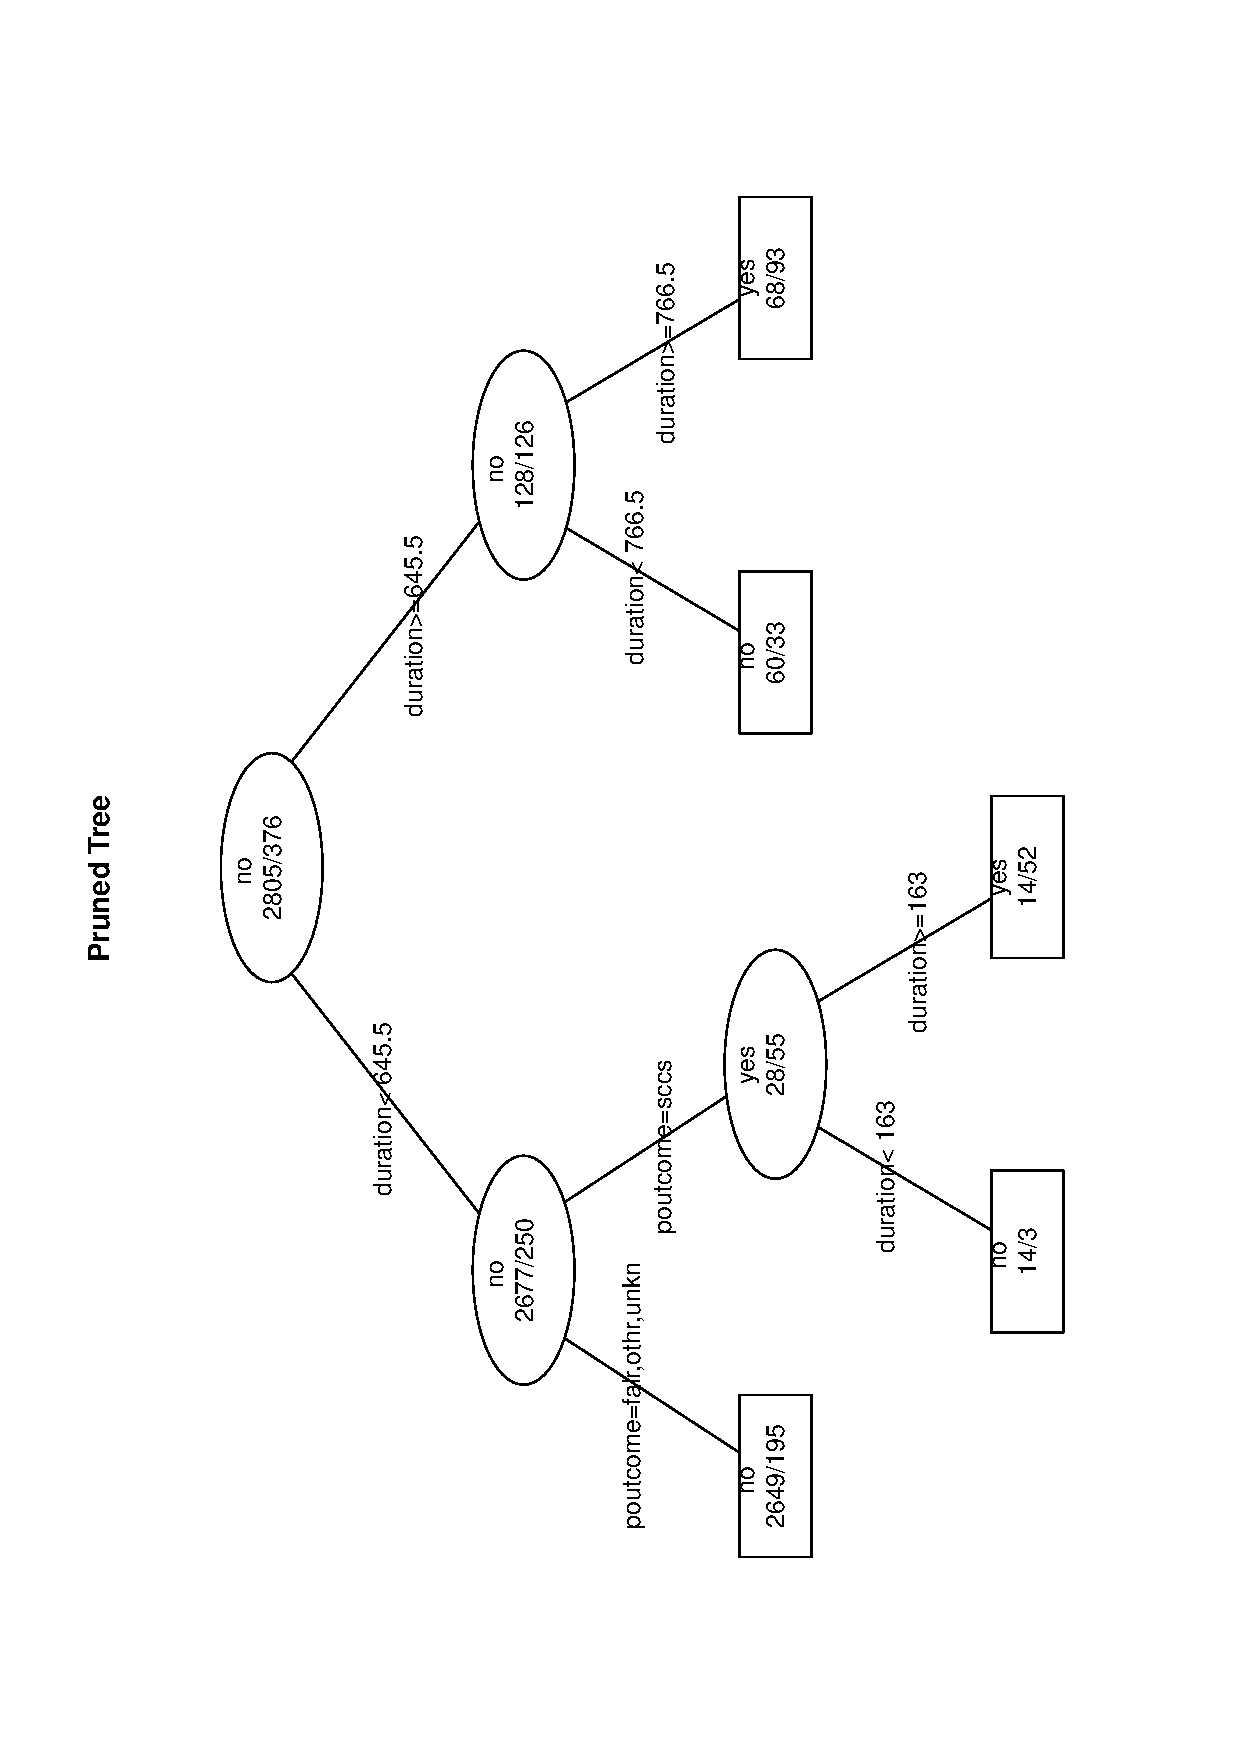
\includegraphics[width=1\columnwidth]{fig/ptree}
\caption{Pruned Tree}
\label{ptree}
\end{figure} 

\subsection{Random Forest}
Bagging and boosting methods can increase the performance of classifiers.
Random forests use a modified tree learning algorithm that selects, at each
candidate split in the learning process, a random subset of the features.
The reason for doing this is the correlation of the trees in an ordinary
bootstrap sample: if one or a few features are very strong predictors for 
the response variable (target output), these features will be selected in
many of the B trees, causing them to become correlated \cite{bryll2003attribute}.
We used random forest classifier as our bagging method to elevate the final
predictions accuracy. We configured the random forest algorithm by setting up
prediction trees range from 10 to 100 to grow in each round. We got the
importance of every predictor by observing the MeanDecreaseGini in Table~\ref
{imp} when we set the number of trees to 100. 


\begin{table*}[!htbp]
\centering
\caption{Importance of Predictors}\label{imp}
\begin{tabular}{ll}
\hline
\hline
Predictor &MeanDecreaseGini\\
  \hline
age         &     81.987620\\
job          &    69.103244\\
marital      &    20.575953\\
education    &    24.121349\\
default      &     2.635483\\
balance      &    85.434797\\
housing      &    13.073510\\
loan         &     6.257758\\
contact      &    16.837081\\
day          &    77.674435\\
month        &   105.590479\\
duration     &   257.728635\\
campaign     &    32.924787\\
pdays        &    39.741963\\
previous     &    22.322606\\
poutcome     &    54.182151\\
\hline
\hline
\end{tabular}
\end{table*}

\subsection{Adaboost}
We adopted Adaboost as our boosting method to train a stronger learner. We 
did 50 iterations in the Adaptive Boosting and the model fitted shows a train
error of 5.5\% which is no doubly a better result than the former decision
tree.

\section{Evaluation}
To evaluate the models fitted using the training data, we tested with the
remaining 30\% data to each model in each round and we adopted the 10-fold 
cross-validation to make the result more convincing.  We demonstrate the
 performance of the models in terms of (1) Average Accuracy, (2) Precision/
 Recall Curves, and (3) ROC curves.

\subsection{Average Accuracy}
Predictive accuracy refers to the ability of the model to correctly predict
the class label of new or previously unseen data. In our models, we get the
average accuracy from 10 rounds of cross-validation and each of them are the
numbers of attributions correctly classified. The average accuracies of the 
(i) Pruned Decision Tree, (ii) Random Forest, and (iii) Adaboost are shown
in Table~\ref{acc}.

According to the table which indicates that the latter two models demonstrate
higher average accuracy, we can conclude with the statement: bagging and 
boosting elevate the performance of the classic decision trees with higher
predictive accuracies.

\begin{table*}[!htbp]
\centering
\caption{Importance of Predictors}\label{imp}
\begin{tabular}{lll}
\hline
\hline
Model& Average Accuracy& Std. Dev. (+/-) \\
  \hline
Decision Tree& 90.15\% & 8.03\%\\
Random Forest& 96.97\% & 0.57\%\\
Adaboost& 96.96\% & 0.62\%\\
\hline
\hline
\end{tabular}
\end{table*}

\subsection{Precision/Recall Curves}
Precision and Recall are two measurements of great importance in data mining
technologies. Precision is the probability that a (randomly selected) 
retrieved document is relevant. Recall is the probability that a (randomly 
selected) relevant document is retrieved in a search. We use Precision/Recall
Curves which is a built-in measure in the ROCR package in R. 

The three curves are depicted in Figure~\ref{PrecRecall}.

\begin{figure} 
  \subfigure[Pruned Tree]{ 
     %% label for first subfigure 
    \begin{minipage}[b]{0.333\textwidth} 
      \centering 
      \includegraphics[width=2in]{fig/precrecall2} 
    \end{minipage}}% 
  \subfigure[Random Forest]{ 
     %% label for second subfigure 
    \begin{minipage}[b]{0.333\textwidth} 
      \centering 
      \includegraphics[width=2in]{fig/precrecallrf} 
    \end{minipage}} 
     \subfigure[Adaboost]{ 
     %% label for second subfigure 
    \begin{minipage}[b]{0.333\textwidth} 
      \centering 
      \includegraphics[width=2in]{fig/precrecall3} 
    \end{minipage}}
  \caption{Precision/Recall Curves} 
   %% label for entire figure 
\end{figure}\label{PrecRecall}

\subsection{ROC Curve}
ROC curve is a graphical plot which illustrates the performance of a binary
classifier system as its discrimination threshold is varied \cite{green1966signal}.
 A ROC space is defined by FPR and TPR as x and y axes respectively, which
depicts relative trade-offs between true positive (benefits) and false 
positive (costs). Since our task is to do a binary classification, we 
adopted this measurement for the evaluation as shown in Figure~\ref{roc}.
As a result, these plots demonstrate that the random forest algorithm
outperforms every other algorithm by a fairly wide margin.


\begin{figure}[!tp]
\centering
\includegraphics[width=1.2\columnwidth]{fig/roc}
\caption{ROC Curves for each model}
\label{roc}
\end{figure}

\section{Conclusion}
In this task, we applied the classic data mining method, decision tree to a
bank marketing dataset that predicts a user will subscribe the deposit or not
based on a set a predictors collected by the contact campaign. We first 
built a full tree by using the Gini Criterion as the goodness of split and 
the CP value as well as the least number to split as the stopping criteria.
We pruned the tree using cross-validation and get a 17 split tree out of a 
47-splits-full tree. We also applied the Random Forest and Adaboost as the 
bagging and boosting methods that assist with the model construction. 

To evaluate the models we construct, we adopted the Average Accuracy, 
Precision/Recall Curves, and ROC curves. Random Forest and Adaboost 
outperform than the classic Decision Tree.




\bibliographystyle{abbrv}
\bibliography{main}
\end{document}